\documentclass[tikz,border=8pt]{standalone}
\usepackage[utf8]{inputenc}
\usepackage[OT4,plmath]{polski}
\begin{document}
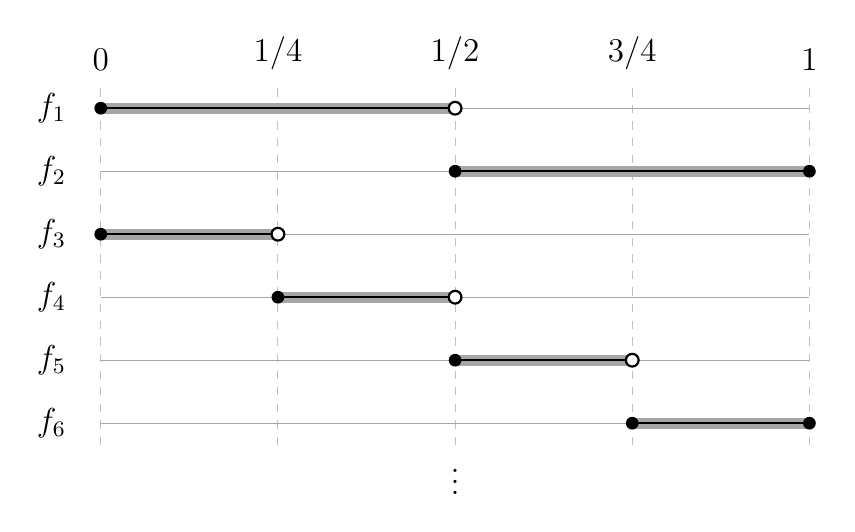
\begin{tikzpicture}[x=9cm,y=0.8cm,>=stealth,font=\large]
  \foreach \pos/\lab in {0/0,0.25/{1/4},0.5/{1/2},0.75/{3/4},1/1} {
    \draw[black!25,dashed] (\pos,0.65) -- (\pos,6.4);
    \node[above] at (\pos,6.45) {$\lab$};
  }
  \foreach \row/\start/\finish/\lab in {6/0/0.5/f_1,5/0.5/1/f_2,4/0/0.25/f_3,3/0.25/0.5/f_4,2/0.5/0.75/f_5,1/0.75/1/f_6} {
    \draw[black!35] (0,\row) -- (1,\row);
    \draw[line width=4pt,black!35] (\start,\row) -- (\finish,\row);
    \draw[thick] (\start,\row) -- (\finish,\row);
    \fill (\start,\row) circle[radius=2.3pt];
    \ifdim\finish pt=1pt
      \fill (\finish,\row) circle[radius=2.3pt];
    \else
      \draw[thick,fill=white] (\finish,\row) circle[radius=2.3pt];
    \fi
    \node[left=9pt] at (0,\row) {$\lab$};
  }
  \node at (0.5,0.2) {$\vdots$};
\end{tikzpicture}
\end{document}
